
\documentclass[11pt]{article}

\usepackage[margin=1in]{geometry}
\usepackage[T1]{fontenc}
\usepackage[utf8]{inputenc}
\usepackage{lmodern}
\usepackage{microtype}
\usepackage{amsmath,amssymb,amsthm,mathtools,bm}
\usepackage{booktabs,array,longtable}
\usepackage{hyperref}
\usepackage{xcolor}
\usepackage[most]{tcolorbox}
\usepackage{tikz}
\usepackage{pgfplots}
\usepackage{tikz-3dplot}
\usepackage{enumitem}
\usepackage{caption}
\usepackage{float}
\usepackage{fancyhdr}
\usepackage{titlesec}

\pgfplotsset{compat=1.18}
\usetikzlibrary{arrows.meta,calc,patterns,decorations.pathreplacing,positioning,3d,backgrounds}

\hypersetup{colorlinks=true, linkcolor=blue!60!black, urlcolor=blue!60!black, citecolor=blue!60!black, pdftitle={Chapter 22. Curl, Divergence, and Surface Integrals}}

\setlength{\headheight}{14pt}
\setlength{\parindent}{0pt}
\setlength{\parskip}{0.65em}
\setlist[itemize]{topsep=2pt,itemsep=2pt}
\setlist[enumerate]{topsep=2pt,itemsep=2pt}

\titleformat{\section}{\large\bfseries}{\thesection}{0.6em}{}
\titleformat{\subsection}{\normalsize\bfseries}{\thesubsection}{0.6em}{}

\pagestyle{fancy}
\fancyhf{}
\lhead{Chapter 22. Curl, Divergence, and Surface Integrals}
\rhead{\thepage}
\renewcommand{\headrulewidth}{0.4pt}

\newtcolorbox{chapteroverviewbox}{colback=blue!4,colframe=blue!50!black,boxrule=0.7pt,arc=2mm,left=2mm,right=2mm,top=1mm,bottom=1mm}
\newtcolorbox{goalbox}{colback=green!4,colframe=green!45!black,title=Learning goals,fonttitle=\bfseries,boxrule=0.7pt,arc=2mm}
\newtcolorbox{notebox}[1][]{colback=blue!3,colframe=blue!50!black,fonttitle=\bfseries,title=#1,boxrule=0.7pt,arc=2mm}
\newtcolorbox{importantbox}[1][]{colback=red!3,colframe=red!60!black,fonttitle=\bfseries,title=#1,boxrule=0.7pt,arc=2mm}
\newtcolorbox{warningbox}[1][]{colback=yellow!8,colframe=orange!75!black,fonttitle=\bfseries,title=#1,boxrule=0.7pt,arc=2mm}

\newtcbtheorem[number within=section]{examplebox}{Example}{enhanced,breakable,colback=white,colframe=blue!60!black,colbacktitle=blue!60!black,fonttitle=\bfseries,boxrule=0.7pt,arc=1.5mm,left=2mm,right=2mm,top=1mm,bottom=1mm}{ex}

\newcommand{\R}{\mathbb R}
\newcommand{\ii}{\mathbf i}
\newcommand{\jj}{\mathbf j}
\newcommand{\kk}{\mathbf k}
\newcommand{\grad}{\nabla}
\newcommand{\dS}{\,dS}
\newcommand{\dA}{\,dA}
\newcommand{\du}{\,du}
\newcommand{\dv}{\,dv}

\begin{document}

\begin{center}
  {\LARGE\bfseries Chapter 22. Curl, Divergence, and Surface Integrals\par}
  \vspace{0.3em}
  {\large Local rotation, local expansion, oriented surfaces, and flux\par}
\end{center}

\begin{chapteroverviewbox}
The previous chapters developed line integrals and Green's theorem. A line integral measures how a scalar or vector field accumulates along a curve. Green's theorem showed that circulation or flux around a closed plane curve can be computed by integrating a local derivative over the enclosed region.

This chapter moves that idea into three-dimensional space. Instead of curves enclosing planar regions, we now study surfaces in space. Instead of asking only how much a vector field pushes along a path, we ask how much it rotates near a point, how much it expands out of a point, and how much it flows through a surface.

The central objects are curl, divergence, scalar surface integrals, and flux integrals. They prepare the way for Stokes' theorem and the divergence theorem.
\end{chapteroverviewbox}

\begin{goalbox}
After studying this chapter, you should be able to:
\begin{enumerate}
  \item compute the curl of a vector field in space;
  \item interpret curl as local rotational tendency;
  \item compute and interpret divergence;
  \item use the identities $\grad\cdot(\grad\times F)=0$ and $\grad\times(\grad f)=0$ when appropriate;
  \item parameterize surfaces and compute tangent vectors;
  \item compute surface area using $|r_u\times r_v|$;
  \item compute scalar surface integrals;
  \item orient a surface and compute flux integrals;
  \item use graph formulas for surface area and flux;
  \item approximate curl, divergence, surface area, and flux numerically.
\end{enumerate}
\end{goalbox}

\begin{notebox}[The main theme]
Curl and divergence are local differential measurements. Surface integrals and flux integrals are global accumulations. The great theorems of vector calculus explain when local rotation or local expansion determines a global boundary integral.
\end{notebox}

\section{The differential operator $\nabla$}

For a scalar function $f(x,y,z)$, the gradient is
\[
\grad f=\langle f_x,f_y,f_z\rangle.
\]
For a vector field
\[
F(x,y,z)=\langle P(x,y,z),Q(x,y,z),R(x,y,z)\rangle,
\]
we use the formal differential operator
\[
\grad=\left\langle \frac{\partial}{\partial x},\frac{\partial}{\partial y},\frac{\partial}{\partial z}\right\rangle.
\]
This notation organizes three operations:
\[
\grad f \quad \text{gradient},\qquad
\grad\cdot F \quad \text{divergence},\qquad
\grad\times F \quad \text{curl}.
\]
The notation is formal: $\grad$ is not an ordinary vector of numbers. Its components are derivative operators.

\section{Curl}

Let $F=\langle P,Q,R\rangle$ be a vector field in space. The \emph{curl} of $F$ is
\[
\grad\times F=\left\langle R_y-Q_z,\; P_z-R_x,\; Q_x-P_y\right\rangle.
\]
Equivalently,
\[
\grad\times F=
\begin{vmatrix}
\ii & \jj & \kk\\
\frac{\partial}{\partial x} & \frac{\partial}{\partial y} & \frac{\partial}{\partial z}\\
P & Q & R
\end{vmatrix}.
\]
Curl measures the infinitesimal tendency of the field to rotate. Its direction is the axis of rotation determined by the right-hand rule, and its magnitude measures the local strength of rotation.

\begin{importantbox}[Curl in the plane]
A two-dimensional vector field $F(x,y)=\langle P(x,y),Q(x,y)\rangle$ can be treated as the three-dimensional field $\langle P,Q,0\rangle$. Then
\[
\grad\times F=\langle 0,0,Q_x-P_y\rangle.
\]
The scalar quantity $Q_x-P_y$ is the scalar curl of the plane field. It is exactly the integrand in Green's theorem in circulation form.
\end{importantbox}

\begin{examplebox}{A rotating field}{rotfield}
Let
\[
F(x,y,z)=\langle -y,x,0\rangle.
\]
Then $P=-y$, $Q=x$, and $R=0$. Hence
\[
\grad\times F=\langle 0-0,\;0-0,
\;1-(-1)\rangle=\langle 0,0,2\rangle.
\]
The field rotates counterclockwise in the $xy$-plane. The curl points in the positive $z$-direction.
\end{examplebox}

\begin{figure}[H]
\centering
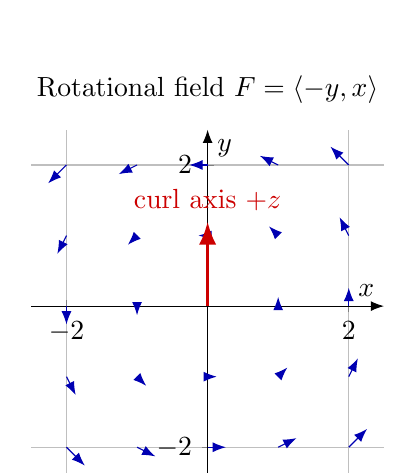
\begin{tikzpicture}
\begin{axis}[
  width=0.66\textwidth,height=0.50\textwidth,
  xmin=-2.5,xmax=2.5,ymin=-2.5,ymax=2.5,
  axis equal image,axis lines=middle,
  xlabel={$x$},ylabel={$y$},grid=both,
  axis line style={-Latex},title={Rotational field $F=\langle -y,x\rangle$}
]
\draw[-Latex,blue!70!black] (axis cs:-2.00,-2.00) -- (axis cs:-1.740,-2.260);
\draw[-Latex,blue!70!black] (axis cs:-2.00,-1.00) -- (axis cs:-1.870,-1.260);
\draw[-Latex,blue!70!black] (axis cs:-2.00,0.00) -- (axis cs:-2.000,-0.260);
\draw[-Latex,blue!70!black] (axis cs:-2.00,1.00) -- (axis cs:-2.130,0.740);
\draw[-Latex,blue!70!black] (axis cs:-2.00,2.00) -- (axis cs:-2.260,1.740);
\draw[-Latex,blue!70!black] (axis cs:-1.00,-2.00) -- (axis cs:-0.740,-2.130);
\draw[-Latex,blue!70!black] (axis cs:-1.00,-1.00) -- (axis cs:-0.870,-1.130);
\draw[-Latex,blue!70!black] (axis cs:-1.00,0.00) -- (axis cs:-1.000,-0.130);
\draw[-Latex,blue!70!black] (axis cs:-1.00,1.00) -- (axis cs:-1.130,0.870);
\draw[-Latex,blue!70!black] (axis cs:-1.00,2.00) -- (axis cs:-1.260,1.870);
\draw[-Latex,blue!70!black] (axis cs:0.00,-2.00) -- (axis cs:0.260,-2.000);
\draw[-Latex,blue!70!black] (axis cs:0.00,-1.00) -- (axis cs:0.130,-1.000);
\draw[-Latex,blue!70!black] (axis cs:0.00,1.00) -- (axis cs:-0.130,1.000);
\draw[-Latex,blue!70!black] (axis cs:0.00,2.00) -- (axis cs:-0.260,2.000);
\draw[-Latex,blue!70!black] (axis cs:1.00,-2.00) -- (axis cs:1.260,-1.870);
\draw[-Latex,blue!70!black] (axis cs:1.00,-1.00) -- (axis cs:1.130,-0.870);
\draw[-Latex,blue!70!black] (axis cs:1.00,0.00) -- (axis cs:1.000,0.130);
\draw[-Latex,blue!70!black] (axis cs:1.00,1.00) -- (axis cs:0.870,1.130);
\draw[-Latex,blue!70!black] (axis cs:1.00,2.00) -- (axis cs:0.740,2.130);
\draw[-Latex,blue!70!black] (axis cs:2.00,-2.00) -- (axis cs:2.260,-1.740);
\draw[-Latex,blue!70!black] (axis cs:2.00,-1.00) -- (axis cs:2.130,-0.740);
\draw[-Latex,blue!70!black] (axis cs:2.00,0.00) -- (axis cs:2.000,0.260);
\draw[-Latex,blue!70!black] (axis cs:2.00,1.00) -- (axis cs:1.870,1.260);
\draw[-Latex,blue!70!black] (axis cs:2.00,2.00) -- (axis cs:1.740,2.260);
\draw[very thick,red!80!black,-Latex] (axis cs:0,0) -- (axis cs:0,1.2) node[above] {curl axis $+z$};
\end{axis}
\end{tikzpicture}
\caption{The field $F=\langle -y,x\rangle$ rotates counterclockwise. Its curl points in the positive $z$-direction.}
\end{figure}

\begin{examplebox}{Curl of a three-dimensional field}{curl3d}
Let
\[
F(x,y,z)=\langle yz,xz,xy+e^z\rangle.
\]
Then $P=yz$, $Q=xz$, and $R=xy+e^z$. We have
\[
R_y=x,\quad Q_z=x,\qquad P_z=y,\quad R_x=y,\qquad Q_x=z,\quad P_y=z.
\]
Hence
\[
\grad\times F=\langle x-x,y-y,z-z\rangle=\langle 0,0,0\rangle.
\]
Indeed, $F=\grad f$ for $f(x,y,z)=xyz+e^z$.
\end{examplebox}

\section{Divergence}

Let $F=\langle P,Q,R\rangle$. The \emph{divergence} of $F$ is the scalar field
\[
\grad\cdot F=P_x+Q_y+R_z.
\]
Divergence measures the local tendency of a vector field to flow outward from a point. Positive divergence indicates source-like behavior, negative divergence indicates sink-like behavior, and zero divergence indicates local incompressibility.

\begin{importantbox}[Divergence is a scalar field]
Curl returns a vector field in three dimensions. Divergence returns a scalar field:
\[
\grad\times F\in\R^3,\qquad \grad\cdot F\in\R.
\]
\end{importantbox}

\begin{examplebox}{A source field and an incompressible rotational field}{divexamples}
For $F(x,y,z)=\langle x,y,z\rangle$,
\[
\grad\cdot F=1+1+1=3.
\]
The field points away from the origin and has positive divergence.

For $F(x,y,z)=\langle -y,x,0\rangle$,
\[
\grad\cdot F=0+0+0=0.
\]
The field rotates, but it does not locally expand or compress volume.
\end{examplebox}

\begin{figure}[H]
\centering
\begin{minipage}{0.48\textwidth}
\centering
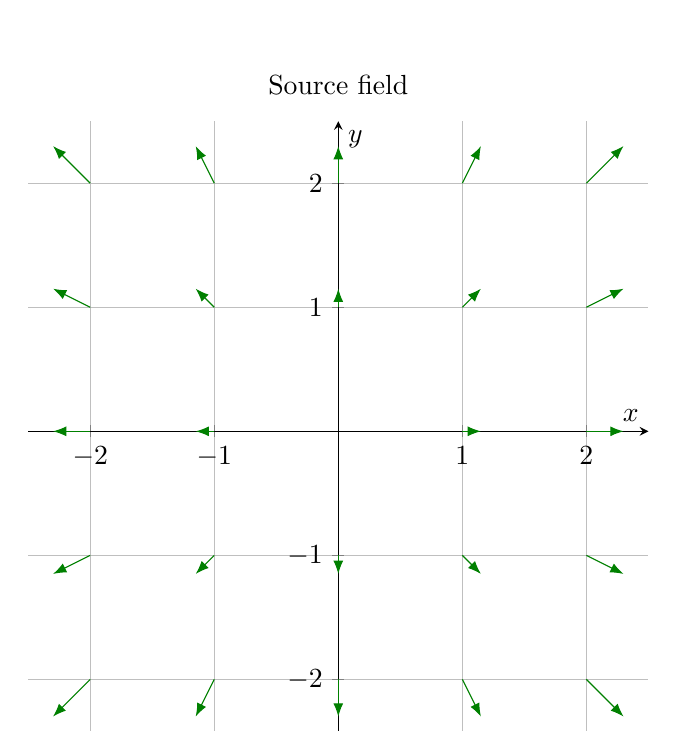
\begin{tikzpicture}
\begin{axis}[width=\textwidth,height=0.78\textwidth,xmin=-2.5,xmax=2.5,ymin=-2.5,ymax=2.5,axis equal image,axis lines=middle,xlabel={$x$},ylabel={$y$},grid=both,title={Source field}]
\draw[-Latex,green!50!black] (axis cs:-2.00,-2.00) -- (axis cs:-2.300,-2.300);
\draw[-Latex,green!50!black] (axis cs:-2.00,-1.00) -- (axis cs:-2.300,-1.150);
\draw[-Latex,green!50!black] (axis cs:-2.00,0.00) -- (axis cs:-2.300,0.000);
\draw[-Latex,green!50!black] (axis cs:-2.00,1.00) -- (axis cs:-2.300,1.150);
\draw[-Latex,green!50!black] (axis cs:-2.00,2.00) -- (axis cs:-2.300,2.300);
\draw[-Latex,green!50!black] (axis cs:-1.00,-2.00) -- (axis cs:-1.150,-2.300);
\draw[-Latex,green!50!black] (axis cs:-1.00,-1.00) -- (axis cs:-1.150,-1.150);
\draw[-Latex,green!50!black] (axis cs:-1.00,0.00) -- (axis cs:-1.150,0.000);
\draw[-Latex,green!50!black] (axis cs:-1.00,1.00) -- (axis cs:-1.150,1.150);
\draw[-Latex,green!50!black] (axis cs:-1.00,2.00) -- (axis cs:-1.150,2.300);
\draw[-Latex,green!50!black] (axis cs:0.00,-2.00) -- (axis cs:0.000,-2.300);
\draw[-Latex,green!50!black] (axis cs:0.00,-1.00) -- (axis cs:0.000,-1.150);
\draw[-Latex,green!50!black] (axis cs:0.00,1.00) -- (axis cs:0.000,1.150);
\draw[-Latex,green!50!black] (axis cs:0.00,2.00) -- (axis cs:0.000,2.300);
\draw[-Latex,green!50!black] (axis cs:1.00,-2.00) -- (axis cs:1.150,-2.300);
\draw[-Latex,green!50!black] (axis cs:1.00,-1.00) -- (axis cs:1.150,-1.150);
\draw[-Latex,green!50!black] (axis cs:1.00,0.00) -- (axis cs:1.150,0.000);
\draw[-Latex,green!50!black] (axis cs:1.00,1.00) -- (axis cs:1.150,1.150);
\draw[-Latex,green!50!black] (axis cs:1.00,2.00) -- (axis cs:1.150,2.300);
\draw[-Latex,green!50!black] (axis cs:2.00,-2.00) -- (axis cs:2.300,-2.300);
\draw[-Latex,green!50!black] (axis cs:2.00,-1.00) -- (axis cs:2.300,-1.150);
\draw[-Latex,green!50!black] (axis cs:2.00,0.00) -- (axis cs:2.300,0.000);
\draw[-Latex,green!50!black] (axis cs:2.00,1.00) -- (axis cs:2.300,1.150);
\draw[-Latex,green!50!black] (axis cs:2.00,2.00) -- (axis cs:2.300,2.300);
\end{axis}
\end{tikzpicture}
\end{minipage}\hfill
\begin{minipage}{0.48\textwidth}
\centering
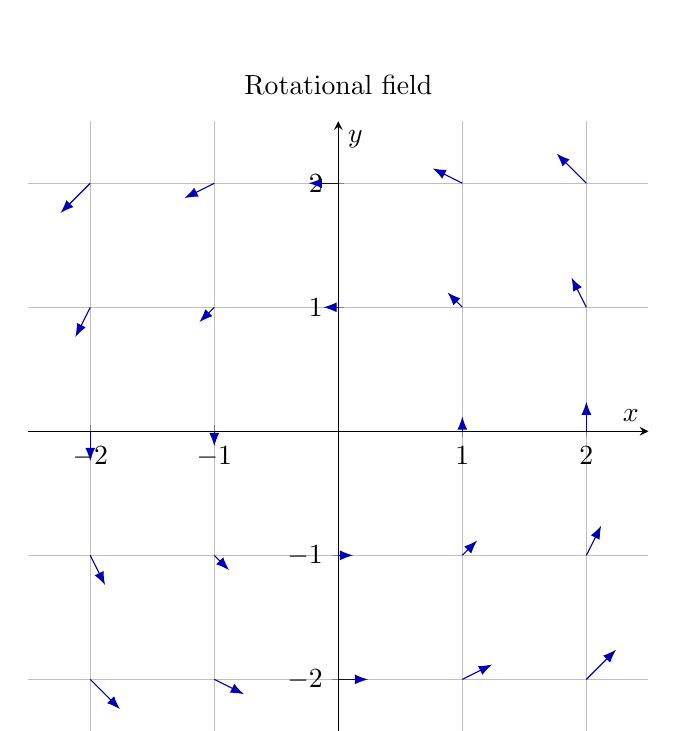
\begin{tikzpicture}
\begin{axis}[width=\textwidth,height=0.78\textwidth,xmin=-2.5,xmax=2.5,ymin=-2.5,ymax=2.5,axis equal image,axis lines=middle,xlabel={$x$},ylabel={$y$},grid=both,title={Rotational field}]
\draw[-Latex,blue!70!black] (axis cs:-2.00,-2.00) -- (axis cs:-1.760,-2.240);
\draw[-Latex,blue!70!black] (axis cs:-2.00,-1.00) -- (axis cs:-1.880,-1.240);
\draw[-Latex,blue!70!black] (axis cs:-2.00,0.00) -- (axis cs:-2.000,-0.240);
\draw[-Latex,blue!70!black] (axis cs:-2.00,1.00) -- (axis cs:-2.120,0.760);
\draw[-Latex,blue!70!black] (axis cs:-2.00,2.00) -- (axis cs:-2.240,1.760);
\draw[-Latex,blue!70!black] (axis cs:-1.00,-2.00) -- (axis cs:-0.760,-2.120);
\draw[-Latex,blue!70!black] (axis cs:-1.00,-1.00) -- (axis cs:-0.880,-1.120);
\draw[-Latex,blue!70!black] (axis cs:-1.00,0.00) -- (axis cs:-1.000,-0.120);
\draw[-Latex,blue!70!black] (axis cs:-1.00,1.00) -- (axis cs:-1.120,0.880);
\draw[-Latex,blue!70!black] (axis cs:-1.00,2.00) -- (axis cs:-1.240,1.880);
\draw[-Latex,blue!70!black] (axis cs:0.00,-2.00) -- (axis cs:0.240,-2.000);
\draw[-Latex,blue!70!black] (axis cs:0.00,-1.00) -- (axis cs:0.120,-1.000);
\draw[-Latex,blue!70!black] (axis cs:0.00,1.00) -- (axis cs:-0.120,1.000);
\draw[-Latex,blue!70!black] (axis cs:0.00,2.00) -- (axis cs:-0.240,2.000);
\draw[-Latex,blue!70!black] (axis cs:1.00,-2.00) -- (axis cs:1.240,-1.880);
\draw[-Latex,blue!70!black] (axis cs:1.00,-1.00) -- (axis cs:1.120,-0.880);
\draw[-Latex,blue!70!black] (axis cs:1.00,0.00) -- (axis cs:1.000,0.120);
\draw[-Latex,blue!70!black] (axis cs:1.00,1.00) -- (axis cs:0.880,1.120);
\draw[-Latex,blue!70!black] (axis cs:1.00,2.00) -- (axis cs:0.760,2.120);
\draw[-Latex,blue!70!black] (axis cs:2.00,-2.00) -- (axis cs:2.240,-1.760);
\draw[-Latex,blue!70!black] (axis cs:2.00,-1.00) -- (axis cs:2.120,-0.760);
\draw[-Latex,blue!70!black] (axis cs:2.00,0.00) -- (axis cs:2.000,0.240);
\draw[-Latex,blue!70!black] (axis cs:2.00,1.00) -- (axis cs:1.880,1.240);
\draw[-Latex,blue!70!black] (axis cs:2.00,2.00) -- (axis cs:1.760,2.240);
\end{axis}
\end{tikzpicture}
\end{minipage}
\caption{A radial source field has positive divergence. A rotational field can have zero divergence but nonzero curl.}
\end{figure}

\section{Two fundamental identities}

For sufficiently smooth functions and fields, two identities occur throughout vector calculus:
\[
\grad\times(\grad f)=0,
\qquad
\grad\cdot(\grad\times F)=0.
\]
The first says that gradient fields have no local rotation. It is the three-dimensional version of the conservative-field test. The second says that a curl field has no local source or sink.

\begin{warningbox}[Smoothness and domain matter]
These identities require enough differentiability. Also, equations such as $\grad\times F=0$ guarantee a global potential only under suitable assumptions on the domain. Holes and singularities can create global circulation even when local curl is zero away from the singularity.
\end{warningbox}

\section{Numerical curl and divergence on a grid}

In applications, a vector field may be sampled rather than given by a formula. For a plane field $F=\langle P,Q\rangle$, finite differences approximate
\[
\grad\cdot F=P_x+Q_y,
\qquad
\operatorname{curl}_z F=Q_x-P_y.
\]
This is used for fluid simulation, weather models, image motion, and learned dynamical systems.

\begin{figure}[H]
\centering
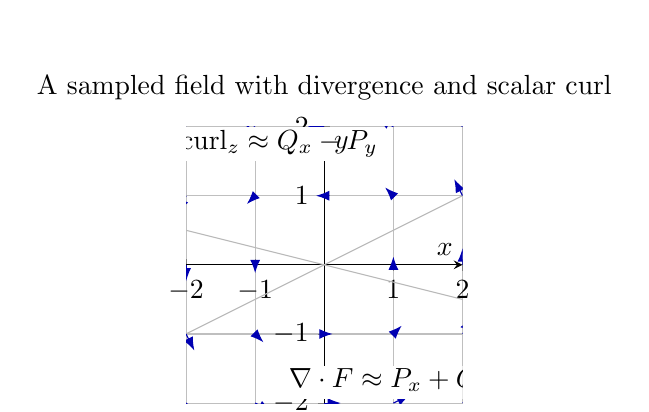
\begin{tikzpicture}
\begin{axis}[
  width=0.70\textwidth,height=0.42\textwidth,
  xmin=-2,xmax=2,ymin=-2,ymax=2,axis equal image,
  axis lines=middle,xlabel={$x$},ylabel={$y$},grid=both,
  title={A sampled field with divergence and scalar curl}
]
\addplot[gray!55,domain=-2:2,samples=80] {-0.25*x};
\addplot[gray!55,domain=-2:2,samples=80] {0.50*x};
\draw[-Latex,blue!70!black] (axis cs:-2.00,-2.00) -- (axis cs:-1.760,-2.240);
\draw[-Latex,blue!70!black] (axis cs:-2.00,-1.00) -- (axis cs:-1.880,-1.240);
\draw[-Latex,blue!70!black] (axis cs:-2.00,0.00) -- (axis cs:-2.000,-0.240);
\draw[-Latex,blue!70!black] (axis cs:-2.00,1.00) -- (axis cs:-2.120,0.760);
\draw[-Latex,blue!70!black] (axis cs:-2.00,2.00) -- (axis cs:-2.240,1.760);
\draw[-Latex,blue!70!black] (axis cs:-1.00,-2.00) -- (axis cs:-0.760,-2.120);
\draw[-Latex,blue!70!black] (axis cs:-1.00,-1.00) -- (axis cs:-0.880,-1.120);
\draw[-Latex,blue!70!black] (axis cs:-1.00,0.00) -- (axis cs:-1.000,-0.120);
\draw[-Latex,blue!70!black] (axis cs:-1.00,1.00) -- (axis cs:-1.120,0.880);
\draw[-Latex,blue!70!black] (axis cs:-1.00,2.00) -- (axis cs:-1.240,1.880);
\draw[-Latex,blue!70!black] (axis cs:0.00,-2.00) -- (axis cs:0.240,-2.000);
\draw[-Latex,blue!70!black] (axis cs:0.00,-1.00) -- (axis cs:0.120,-1.000);
\draw[-Latex,blue!70!black] (axis cs:0.00,1.00) -- (axis cs:-0.120,1.000);
\draw[-Latex,blue!70!black] (axis cs:0.00,2.00) -- (axis cs:-0.240,2.000);
\draw[-Latex,blue!70!black] (axis cs:1.00,-2.00) -- (axis cs:1.240,-1.880);
\draw[-Latex,blue!70!black] (axis cs:1.00,-1.00) -- (axis cs:1.120,-0.880);
\draw[-Latex,blue!70!black] (axis cs:1.00,0.00) -- (axis cs:1.000,0.120);
\draw[-Latex,blue!70!black] (axis cs:1.00,1.00) -- (axis cs:0.880,1.120);
\draw[-Latex,blue!70!black] (axis cs:1.00,2.00) -- (axis cs:0.760,2.120);
\draw[-Latex,blue!70!black] (axis cs:2.00,-2.00) -- (axis cs:2.240,-1.760);
\draw[-Latex,blue!70!black] (axis cs:2.00,-1.00) -- (axis cs:2.120,-0.760);
\draw[-Latex,blue!70!black] (axis cs:2.00,0.00) -- (axis cs:2.000,0.240);
\draw[-Latex,blue!70!black] (axis cs:2.00,1.00) -- (axis cs:1.880,1.240);
\draw[-Latex,blue!70!black] (axis cs:2.00,2.00) -- (axis cs:1.760,2.240);
\node[fill=white,inner sep=1.2pt] at (axis cs:-0.65,1.75) {$\operatorname{curl}_z\approx Q_x-P_y$};
\node[fill=white,inner sep=1.2pt] at (axis cs:0.95,-1.70) {$\grad\cdot F\approx P_x+Q_y$};
\end{axis}
\end{tikzpicture}
\caption{Finite differences approximate divergence and scalar curl from neighboring values on a grid.}
\end{figure}

\section{Surfaces and parameterizations}

A curve is described by one parameter:
\[
r(t)=\langle x(t),y(t),z(t)\rangle.
\]
A surface is described by two parameters:
\[
r(u,v)=\langle x(u,v),y(u,v),z(u,v)\rangle,\qquad (u,v)\in D.
\]
The parameter domain $D$ lies in the $uv$-plane. The map $r$ bends and stretches this flat parameter region into a surface $S$ in space.

For a parameterized surface, the tangent vectors are
\[
r_u=\frac{\partial r}{\partial u},\qquad r_v=\frac{\partial r}{\partial v}.
\]
The cross product $r_u\times r_v$ is normal to the surface. Its magnitude gives the local area scaling factor:
\[
dS=|r_u\times r_v|\du\dv.
\]

\begin{figure}[H]
\centering
\tdplotsetmaincoords{68}{115}
\begin{tikzpicture}[tdplot_main_coords,scale=1.15]
\draw[-Latex,thick] (-2.2,0,0)--(2.4,0,0) node[below] {$x$};
\draw[-Latex,thick] (0,-2.2,0)--(0,2.4,0) node[right] {$y$};
\draw[-Latex,thick] (0,0,0)--(0,0,2.2) node[right] {$z$};
\foreach \r in {0.4,0.8,1.2,1.6} {\draw[blue!40] plot[domain=0:360,samples=80] ({\r*cos(\x)},{\r*sin(\x)},{0.14*\r*\r});}
\foreach \a in {0,45,90,135,180,225,270,315} {\draw[blue!35] plot[domain=0:1.7,samples=60] ({\x*cos(\a)},{\x*sin(\a)},{0.14*\x*\x});}
\coordinate (P) at (1,0.7,0.209);
\draw[very thick,red!80!black,-Latex] (P)--++(0.9,0,0.25) node[above] {$r_u$};
\draw[very thick,green!50!black,-Latex] (P)--++(0,0.9,0.25) node[right] {$r_v$};
\draw[very thick,purple!80!black,-Latex] (P)--++(-0.45,-0.32,1.0) node[above] {$r_u\times r_v$};
\node[fill=white,inner sep=1.2pt] at (0.2,-1.7,1.2) {normal and area scale};
\end{tikzpicture}
\caption{For a parameterized surface, $r_u\times r_v$ gives a normal direction and the local area scale.}
\end{figure}

\section{Surface area}

The area of a parameterized surface $r(u,v)$, $(u,v)\in D$, is
\[
A(S)=\iint_D |r_u\times r_v|\dA.
\]
This is the surface analog of arc length. For curves, $|r'(t)|$ measures how much the parameter stretches length. For surfaces, $|r_u\times r_v|$ measures how much the two-parameter map stretches area.

\subsection*{Graph surfaces}
If a surface is a graph $z=g(x,y)$ over $D$, parameterize it as
\[
r(x,y)=\langle x,y,g(x,y)\rangle.
\]
Then
\[
r_x=\langle 1,0,g_x\rangle,\qquad r_y=\langle 0,1,g_y\rangle,
\]
so
\[
r_x\times r_y=\langle -g_x,-g_y,1\rangle.
\]
Therefore
\[
dS=\sqrt{1+g_x^2+g_y^2}\dA,
\qquad
A(S)=\iint_D \sqrt{1+g_x^2+g_y^2}\dA.
\]

\begin{examplebox}{Area of a plane patch}{planepatch}
Find the area of the part of the plane
\[
z=8+2x+5y
\]
above the rectangle $0\le x\le 3$, $1\le y\le 6$.
Here $g_x=2$ and $g_y=5$, so
\[
\sqrt{1+g_x^2+g_y^2}=\sqrt{1+4+25}=\sqrt{30}.
\]
The rectangle has area $15$, so
\[
A(S)=15\sqrt{30}.
\]
\end{examplebox}

\section{Scalar surface integrals}

If $f(x,y,z)$ is a scalar function defined on a surface $S$, then the scalar surface integral is
\[
\iint_S f(x,y,z)\dS.
\]
For a parameterized surface $r(u,v)$,
\[
\iint_S f\dS=\iint_D f(r(u,v))|r_u\times r_v|\du\dv.
\]
If $f$ is a surface density, this integral gives total mass. If $f=1$, it gives surface area.

\begin{examplebox}{Surface integral over a paraboloid}{paraboloidintegral}
Let $S$ be the graph $z=x^2+y^2$ over the disk $x^2+y^2\le 1$. Compute
\[
\iint_S z\dS.
\]
Since $g(x,y)=x^2+y^2$, we have $g_x=2x$ and $g_y=2y$, so
\[
dS=\sqrt{1+4x^2+4y^2}\dA.
\]
The integral becomes
\[
\iint_D (x^2+y^2)\sqrt{1+4x^2+4y^2}\dA.
\]
In polar coordinates,
\[
\iint_S z\dS=\int_0^{2\pi}\int_0^1 r^2\sqrt{1+4r^2}\,r\,dr\,d\theta
=2\pi\int_0^1 r^3\sqrt{1+4r^2}\,dr.
\]
\end{examplebox}

\begin{figure}[H]
\centering
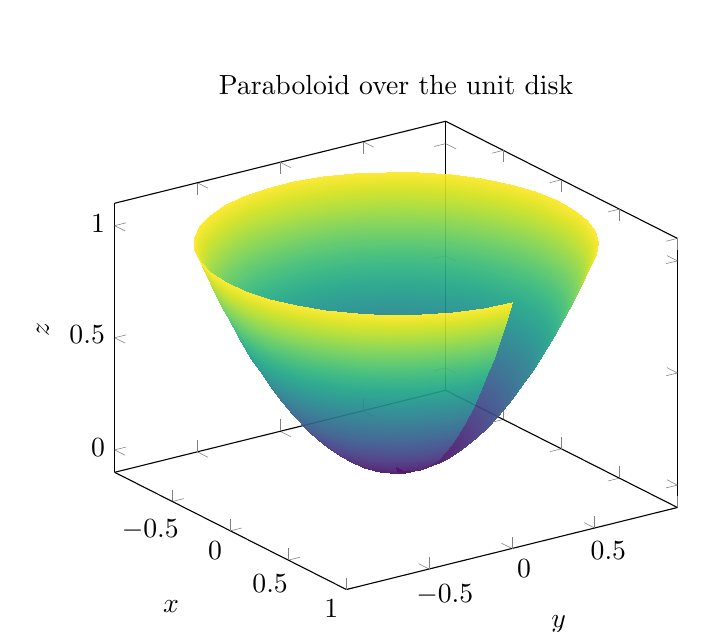
\begin{tikzpicture}
\begin{axis}[
  width=0.72\textwidth,view={55}{28},
  xlabel={$x$},ylabel={$y$},zlabel={$z$},
  domain=0:1,y domain=0:360,samples=20,samples y=40,
  colormap/viridis,title={Paraboloid over the unit disk}
]
\addplot3[surf,shader=interp,opacity=0.92] ({x*cos(y)},{x*sin(y)},{x^2});
\end{axis}
\end{tikzpicture}
\caption{A scalar surface integral accumulates density over a curved surface. Here the density is $f(x,y,z)=z$ on $z=x^2+y^2$.}
\end{figure}

\section{Orientation of surfaces}

A surface is \emph{orientable} if it is possible to choose a continuous unit normal vector $n$ at every point of the surface. Choosing one of the two possible normal directions gives an \emph{orientation}.

For a parameterized surface $r(u,v)$, the vector $r_u\times r_v$ defines one orientation. Reversing the parameter order changes the normal direction:
\[
r_v\times r_u=-(r_u\times r_v).
\]
For a closed surface, the standard orientation is outward. For an open surface, the orientation must be specified, for example upward, downward, outward, or inward.

\begin{warningbox}[Orientation affects flux]
Scalar surface integrals do not depend on orientation because $dS$ is positive. Flux integrals do depend on orientation because changing $n$ to $-n$ changes the sign of $F\cdot n$.
\end{warningbox}

\section{Flux integrals}

Let $F$ be a vector field and let $S$ be an oriented surface with unit normal vector $n$. The \emph{flux} of $F$ through $S$ is
\[
\iint_S F\cdot n\dS.
\]
This measures the net amount of the field passing through the surface in the chosen normal direction.

Using a parameterization $r(u,v)$, we have
\[
n\dS=(r_u\times r_v)\du\dv
\]
for the orientation determined by $r_u\times r_v$. Therefore
\[
\iint_S F\cdot n\dS=\iint_D F(r(u,v))\cdot(r_u\times r_v)\du\dv.
\]

\subsection*{Graph formula for flux}
Suppose $S:z=g(x,y)$ over $D$, with upward orientation. Then
\[
r_x\times r_y=\langle -g_x,-g_y,1\rangle.
\]
If $F=\langle P,Q,R\rangle$, then
\[
\iint_S F\cdot n\dS=\iint_D (-Pg_x-Qg_y+R)\dA,
\]
where $P,Q,R$ are evaluated at $(x,y,g(x,y))$. For downward orientation, the sign changes.

\begin{examplebox}{Flux through a graph}{fluxgraph}
Let $F(x,y,z)=\langle x,y,z\rangle$, and let $S$ be the upper paraboloid
\[
z=1-x^2-y^2,\qquad x^2+y^2\le 1,
\]
with upward orientation. Here $g_x=-2x$ and $g_y=-2y$. The upward flux integrand is
\[
-Pg_x-Qg_y+R=-x(-2x)-y(-2y)+(1-x^2-y^2)=1+x^2+y^2.
\]
Therefore
\[
\iint_S F\cdot n\dS=\iint_D (1+x^2+y^2)\dA.
\]
In polar coordinates,
\[
\int_0^{2\pi}\int_0^1 (1+r^2)r\,dr\,d\theta
=2\pi\left[\frac{r^2}{2}+\frac{r^4}{4}\right]_0^1
=\frac{3\pi}{2}.
\]
\end{examplebox}

\begin{figure}[H]
\centering
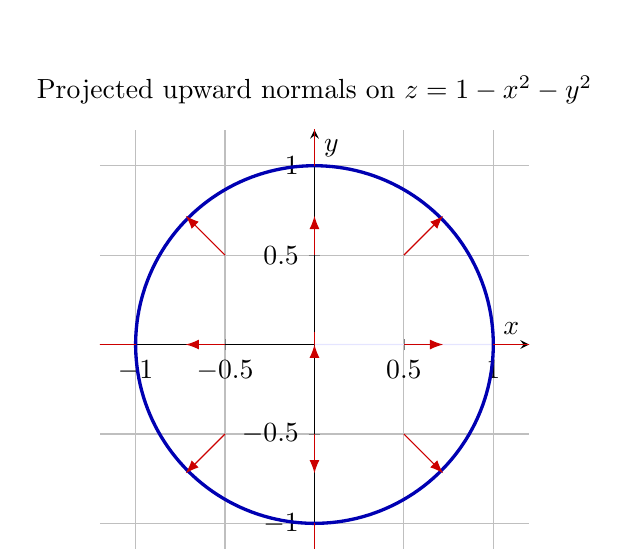
\begin{tikzpicture}
\begin{axis}[
  width=0.58\textwidth,height=0.58\textwidth,
  xmin=-1.2,xmax=1.2,ymin=-1.2,ymax=1.2,
  axis equal image,axis lines=middle,xlabel={$x$},ylabel={$y$},grid=both,
  title={Projected upward normals on $z=1-x^2-y^2$}
]
\addplot[blue!10,domain=0:360,samples=180] ({cos(x)},{sin(x)}) -- (axis cs:0,0) -- cycle;
\addplot[blue!70!black,very thick,domain=0:360,samples=180] ({cos(x)},{sin(x)});
\draw[-Latex,red!80!black] (axis cs:-1.00,0.00) -- (axis cs:-1.440,0.000);
\draw[-Latex,red!80!black] (axis cs:-0.50,-0.50) -- (axis cs:-0.720,-0.720);
\draw[-Latex,red!80!black] (axis cs:-0.50,0.00) -- (axis cs:-0.720,0.000);
\draw[-Latex,red!80!black] (axis cs:-0.50,0.50) -- (axis cs:-0.720,0.720);
\draw[-Latex,red!80!black] (axis cs:0.00,-1.00) -- (axis cs:0.000,-1.440);
\draw[-Latex,red!80!black] (axis cs:0.00,-0.50) -- (axis cs:0.000,-0.720);
\draw[-Latex,red!80!black] (axis cs:0.00,0.00) -- (axis cs:0.000,0.000);
\draw[-Latex,red!80!black] (axis cs:0.00,0.50) -- (axis cs:0.000,0.720);
\draw[-Latex,red!80!black] (axis cs:0.00,1.00) -- (axis cs:0.000,1.440);
\draw[-Latex,red!80!black] (axis cs:0.50,-0.50) -- (axis cs:0.720,-0.720);
\draw[-Latex,red!80!black] (axis cs:0.50,0.00) -- (axis cs:0.720,0.000);
\draw[-Latex,red!80!black] (axis cs:0.50,0.50) -- (axis cs:0.720,0.720);
\draw[-Latex,red!80!black] (axis cs:1.00,0.00) -- (axis cs:1.440,0.000);
\end{axis}
\end{tikzpicture}
\caption{For the upward-oriented graph $z=1-x^2-y^2$, the projected normal arrows in the $xy$-plane point outward and the normal has positive $z$-component.}
\end{figure}

\section{Flux through standard surfaces}

\subsection*{Sphere}
The sphere of radius $a$ centered at the origin can be parameterized by
\[
r(\phi,\theta)=\langle a\sin\phi\cos\theta,
 a\sin\phi\sin\theta,
 a\cos\phi\rangle,
\qquad
0\le\phi\le\pi,
\quad 0\le\theta\le2\pi.
\]
The outward unit normal is
\[
n=\frac1a\langle x,y,z\rangle.
\]
If $F=\langle x,y,z\rangle$, then on the sphere,
\[
F\cdot n=\langle x,y,z\rangle\cdot \frac1a\langle x,y,z\rangle
=\frac{x^2+y^2+z^2}a=a.
\]
Since the surface area is $4\pi a^2$, the flux is
\[
\iint_S F\cdot n\dS=a(4\pi a^2)=4\pi a^3.
\]
For the sphere $x^2+y^2+z^2=4$, $a=2$, so the flux is $32\pi$.

\begin{figure}[H]
\centering
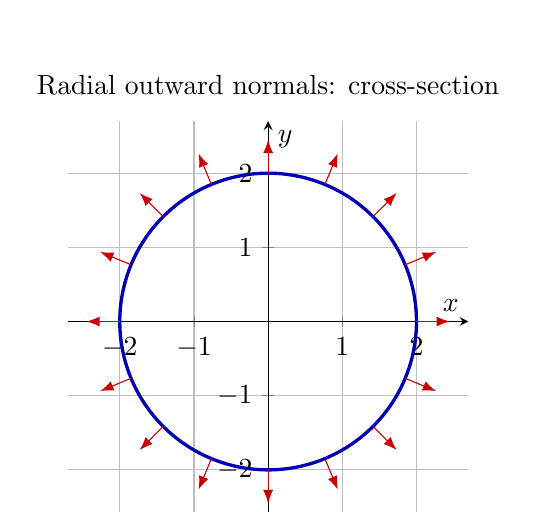
\begin{tikzpicture}
\begin{axis}[width=0.55\textwidth,height=0.55\textwidth,xmin=-2.7,xmax=2.7,ymin=-2.7,ymax=2.7,axis equal image,axis lines=middle,xlabel={$x$},ylabel={$y$},grid=both,title={Radial outward normals: cross-section}]
\addplot[very thick,blue!70!black,domain=0:360,samples=240] ({2*cos(x)},{2*sin(x)});
\draw[-Latex,red!80!black] (axis cs:2.000,0.000) -- (axis cs:2.450,0.000);
\draw[-Latex,red!80!black] (axis cs:1.848,0.765) -- (axis cs:2.264,0.938);
\draw[-Latex,red!80!black] (axis cs:1.414,1.414) -- (axis cs:1.732,1.732);
\draw[-Latex,red!80!black] (axis cs:0.765,1.848) -- (axis cs:0.938,2.264);
\draw[-Latex,red!80!black] (axis cs:0.000,2.000) -- (axis cs:0.000,2.450);
\draw[-Latex,red!80!black] (axis cs:-0.765,1.848) -- (axis cs:-0.938,2.264);
\draw[-Latex,red!80!black] (axis cs:-1.414,1.414) -- (axis cs:-1.732,1.732);
\draw[-Latex,red!80!black] (axis cs:-1.848,0.765) -- (axis cs:-2.264,0.938);
\draw[-Latex,red!80!black] (axis cs:-2.000,0.000) -- (axis cs:-2.450,0.000);
\draw[-Latex,red!80!black] (axis cs:-1.848,-0.765) -- (axis cs:-2.264,-0.938);
\draw[-Latex,red!80!black] (axis cs:-1.414,-1.414) -- (axis cs:-1.732,-1.732);
\draw[-Latex,red!80!black] (axis cs:-0.765,-1.848) -- (axis cs:-0.938,-2.264);
\draw[-Latex,red!80!black] (axis cs:-0.000,-2.000) -- (axis cs:-0.000,-2.450);
\draw[-Latex,red!80!black] (axis cs:0.765,-1.848) -- (axis cs:0.938,-2.264);
\draw[-Latex,red!80!black] (axis cs:1.414,-1.414) -- (axis cs:1.732,-1.732);
\draw[-Latex,red!80!black] (axis cs:1.848,-0.765) -- (axis cs:2.264,-0.938);
\end{axis}
\end{tikzpicture}
\caption{For a sphere centered at the origin, outward normals are radial. The cross-section shows the same orientation idea.}
\end{figure}

\subsection*{Cylinder}
A circular cylinder of radius $a$ can be parameterized by
\[
r(\theta,z)=\langle a\cos\theta,a\sin\theta,z\rangle.
\]
Then
\[
r_\theta=\langle -a\sin\theta,a\cos\theta,0\rangle,
\qquad
r_z=\langle 0,0,1\rangle.
\]
The cross product
\[
r_z\times r_\theta=\langle -a\cos\theta,-a\sin\theta,0\rangle
\]
points inward, while
\[
r_\theta\times r_z=\langle a\cos\theta,a\sin\theta,0\rangle
\]
points outward. Always check orientation.

\section{Numerical surface integration}

For computational work, a parameterized surface integral is usually approximated by sampling a grid in parameter space. If $r(u,v)$, $(u,v)\in D$, then
\[
\iint_S f\dS\approx \sum_{i,j} f(r(u_i,v_j))|r_u(u_i,v_j)\times r_v(u_i,v_j)|\Delta u\Delta v.
\]
Similarly,
\[
\iint_S F\cdot n\dS\approx \sum_{i,j} F(r(u_i,v_j))\cdot(r_u(u_i,v_j)\times r_v(u_i,v_j))\Delta u\Delta v.
\]

\begin{figure}[H]
\centering
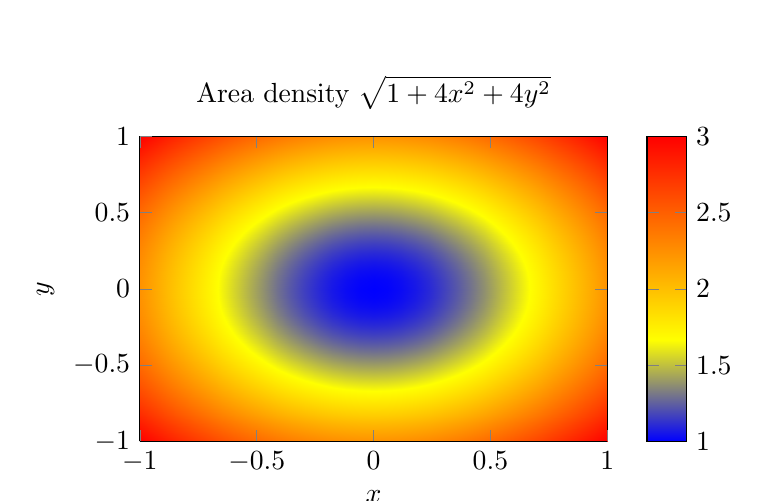
\begin{tikzpicture}
\begin{axis}[
  width=0.62\textwidth,height=0.45\textwidth,
  view={0}{90}, colorbar,
  xlabel={$x$},ylabel={$y$},
  domain=-1:1,y domain=-1:1,samples=35,samples y=35,
  title={Area density $\sqrt{1+4x^2+4y^2}$}
]
\addplot3[surf,shader=interp] {sqrt(1+4*x^2+4*y^2)};
\end{axis}
\end{tikzpicture}
\caption{Numerical surface integration samples the parameter domain and multiplies by the local area scale.}
\end{figure}

The plot shows the area-density factor for $z=x^2+y^2$ over a square. Summing this density over a fine grid is a Riemann-sum approximation to surface area.

\section{Curl, divergence, and flux in applied modeling}

\subsection*{Fluid velocity fields}
If $F$ is a fluid velocity field, then $\grad\times F$ measures local swirling, $\grad\cdot F$ measures local expansion or compression, and $\iint_S F\cdot n\dS$ measures the rate of flow through a surface. These ideas appear in incompressible flow, fluid simulation, weather models, and diffusion processes.

\subsection*{Probability flow}
In probability and statistics, a time-dependent density can move under a velocity field. Divergence helps describe whether probability mass is locally spreading or concentrating. In continuous normalizing flows and score-based generative modeling, vector fields and Jacobians are central tools.

\subsection*{Optimization and machine learning}
Gradient descent is driven by a vector field $-\grad L$. Such a field has zero curl when $L$ is smooth. More general training dynamics may include momentum, stochastic noise, constraints, or game-theoretic interactions. These dynamics can show rotational behavior, naturally detected by curl-like measurements.

\subsection*{Geometry and data}
Surface integrals appear when data lie on curved manifolds rather than flat Euclidean spaces. Area elements and Jacobian factors explain why densities change under parameterization and why sampling uniformly in parameter coordinates does not always sample uniformly on a surface.

\section{Common mistakes}

\begin{enumerate}
  \item Forgetting that curl is a vector in space. In three dimensions, $\grad\times F$ has three components.
  \item Confusing scalar curl with full curl. In the plane, $Q_x-P_y$ is the $z$-component of the three-dimensional curl of $\langle P,Q,0\rangle$.
  \item Forgetting the area factor. The factor $|r_u\times r_v|$ is essential in a surface integral.
  \item Using the wrong orientation. Flux changes sign when the normal direction is reversed.
  \item Using graph formulas outside their setting. The formula for $z=g(x,y)$ applies only when the surface is represented as a graph over the $xy$-plane.
  \item Treating $dS$ like $dA$. For curved surfaces, $dS$ includes an area-stretching factor.
\end{enumerate}

\section{Chapter exercises}

\subsection*{Conceptual exercises}
\begin{enumerate}
  \item Explain the difference between curl and divergence.
  \item Give an example of a vector field with nonzero curl and zero divergence.
  \item Give an example of a vector field with zero curl and nonzero divergence.
  \item Explain why scalar surface integrals do not depend on orientation but flux integrals do.
  \item What does the vector $r_u\times r_v$ represent geometrically?
  \item Why does reversing the order of the cross product reverse the orientation?
  \item Explain why $\grad\times(\grad f)=0$ should be expected geometrically.
  \item Explain why $\grad\cdot(\grad\times F)=0$ suggests that curl fields have no sources or sinks.
\end{enumerate}

\subsection*{Computational exercises}
\begin{enumerate}[start=9]
  \item Compute the curl of $F(x,y,z)=\langle xz,yz,xy\rangle$.
  \item Compute the divergence of $F(x,y,z)=\langle x^2y,y^2z,z^2x\rangle$.
  \item Determine whether $F(x,y,z)=\langle yz,xz,xy\rangle$ has zero curl.
  \item Let $F(x,y,z)=\langle -y,x,z\rangle$. Compute $\grad\times F$ and $\grad\cdot F$.
  \item Let $S$ be the graph $z=x^2+y^2$ over $0\le x\le 1$, $0\le y\le 1$. Set up the surface area integral.
  \item Compute the area of the plane $z=1+2x-2y$ above the rectangle $0\le x\le 3$, $0\le y\le 2$.
  \item Let $S$ be the sphere of radius $3$ centered at the origin. Compute the outward flux of $F=\langle x,y,z\rangle$ through $S$.
  \item Let $S$ be the graph $z=4-x-y$ over the triangle with vertices $(0,0)$, $(1,0)$, and $(0,1)$. Compute the upward flux of $F=\langle 0,0,z\rangle$ through $S$.
  \item Parameterize the cylinder $x^2+y^2=9$, $0\le z\le 4$, and compute $|r_\theta\times r_z|$.
  \item Let $r(u,v)=\langle u,v,u^2-v^2\rangle$, $0\le u\le 1$, $0\le v\le 1$. Compute $r_u\times r_v$ and set up the surface area integral.
\end{enumerate}

\subsection*{Applied and computational exercises}
\begin{enumerate}[start=19]
  \item Approximate the surface area of $z=\sin(xy)$ over $[-1,1]\times[-1,1]$.
  \item Approximate the flux of $F=\langle x,y,z\rangle$ through the upward-oriented graph $z=1-x^2-y^2$ over the unit disk.
  \item Suppose a measured two-dimensional velocity field has approximately zero divergence but nonzero scalar curl. Give an applied interpretation.
  \item Suppose a learned dynamical system in parameter space has visible rotational motion around a point. Which derivative measurement from this chapter would detect that behavior?
  \item A surface is parameterized by a neural network $r(u,v)$. Explain why $|r_u\times r_v|$ is the correct local area distortion factor.
  \item In a probability flow model, why is divergence related to local density change?
\end{enumerate}

\section{Chapter summary}

This chapter introduced the local derivative operations and surface integrals needed for the final theorems of vector calculus.
\begin{itemize}
  \item Curl measures local rotation.
  \item Divergence measures local source or sink behavior.
  \item In the plane, scalar curl is $Q_x-P_y$.
  \item In space, curl is $\grad\times F$ and divergence is $\grad\cdot F$.
  \item The identity $\grad\times(\grad f)=0$ says gradient fields have no local rotation.
  \item The identity $\grad\cdot(\grad\times F)=0$ says curl fields have no local source or sink.
  \item A parameterized surface $r(u,v)$ has tangent vectors $r_u$ and $r_v$.
  \item The vector $r_u\times r_v$ gives a normal direction and an area scale.
  \item Scalar surface integrals accumulate scalar quantities over curved surfaces.
  \item Flux integrals measure how much a vector field passes through an oriented surface.
  \item Orientation matters for flux but not for scalar surface integrals.
\end{itemize}

The next chapter uses these tools to state and apply Stokes' theorem and the divergence theorem, the three-dimensional successors of Green's theorem.

\end{document}
